\documentclass{beamer}

\usetheme[progressbar=frametitle]{metropolis}
\usepackage{appendixnumberbeamer}

\usepackage{booktabs}
\usepackage[scale=2]{ccicons}

\usepackage{pgfplots}
\usepgfplotslibrary{dateplot}

\usepackage{xspace}
\newcommand{\themename}{\textbf{\textsc{metropolis}}\xspace}

\usepackage{amsthm, amsmath, amsfonts, amssymb}
\usepackage{relsize}
\usepackage{graphicx}
\usepackage{subcaption}
\usepackage{bm}
\usepackage[english]{babel}
\usepackage{booktabs}
\usepackage{mathtools}
\usepackage{algorithm}
\usepackage{algpseudocode}
\usepackage[parfill]{parskip}

%Define theorem formatting

\newcommand{\R}{\mathbb{R}}
\newcommand{\C}{\mathbb{C}}
\newcommand{\N}{\mathbb{N}}
\newcommand{\Z}{\mathbb{Z}}
\newcommand{\Q}{\mathbb{Q}}
\newcommand{\E}{\mathbb{E}}
\newcommand{\Hom}{\textbf{\text{Hom}}}
\newcommand{\PP}{\textbf{P}}
\newcommand{\SPACE}{\textbf{SPACE}}
\newcommand{\NP}{\textbf{NP}}
\newcommand{\POS}{\mathcal{P}}
\newcommand{\SAT}{\textbf{SAT}}
\newcommand{\pard}[2]{\frac{\partial #1}{\partial #2}}
\DeclareMathOperator*{\argmin}{arg\,min}
\DeclareMathOperator*{\argmax}{arg\,max}
\DeclareMathOperator*{\diag}{diag}
\DeclareMathOperator*{\supp}{supp}
\DeclareMathOperator{\SDP}{SDP}
\DeclareMathOperator{\CUT}{MAXCUT}
\DeclareMathOperator{\conv}{\operatorname{conv}}
\DeclareMathOperator{\FW}{FW}
\DeclareMathOperator{\tr}{tr}
\DeclareMathOperator{\rank}{rank}
\newcommand{\st}{{\text{ s.t. }}}
\newcommand{\Sym}{\R^{n\times n}_{sym}}
\renewcommand\top[2]{\genfrac{}{}{0pt}{}{#1}{#2}}
\newcommand\twoline[2]{\genfrac{}{}{0pt}{}{#1}{#2}}

\colorlet{shadecolor}{gray!70}
\setbeamercolor{block body}{bg=shadecolor!30,fg=black}


\title{Quadratic Programs with Sparsity Constraints}
\author{Kevin Shu\inst{1}}
\institute{\inst{1} Georgia Institute of Technology}
\date{}

\begin{document}
\frame{\titlepage}
\begin{frame}
    \centering
    \huge
    {\color{gray}Sparse Quadratic Programming}
\end{frame}
\begin{frame}
\frametitle{Sparse Quadratic Programming}
\begin{block}{Sparse QCQP}
    \begin{equation*}
        \begin{aligned}
            \max\quad & x^{\intercal}A_0x\\
            \st & x^{\intercal}A_1x = 1\\
                &|\supp(x)| \le k
        \end{aligned}
    \end{equation*}
\end{block}

    $A_0, A_1$ are symmetric, and $x \in \R^n$. 
    \[
        \supp(x) = \{i : x_i \neq 0\}.
    \]

\end{frame}
\begin{block}{Sparse QCQP}
    \begin{equation*}
        \max_{S \subseteq [n]}
        \begin{aligned}
            \max\quad & x^{\intercal}A_0x\\
            \st & x^{\intercal}A_1x = 1\\
                &x \in \R^S
        \end{aligned}
    \end{equation*}
\end{block}
\end{frame}
\begin{frame}
    \frametitle{Example}
    \begin{block}{Sparse Linear Regression}
        \begin{equation*}
            \begin{aligned}
            \min & \|Ax - b\|_2^2\\
            \st & |\supp(x)| \le k.
            \end{aligned}
        \end{equation*}
    \end{block}
\end{frame}
\begin{frame}
    \frametitle{Example}
    \begin{figure}[h]
        \centering
        \includegraphics[width=\linewidth]{slide3.jpg}
    \end{figure}
\end{frame}
\begin{frame}
    \frametitle{Example}
    Sparse regression is a sparse QCQP where
    \[
        A_0 = A^{\intercal}bb^{\intercal}A
    \]
    \[
        A_1 = A^{\intercal}A
    \]
\end{frame}
\begin{frame}
    \frametitle{Another Example}
    \begin{block}{Sparse Maximum Eigenvalue}
        \begin{equation*}
            \begin{aligned}
                \max\quad & x^{\intercal}Ax\\
                \st & x^{\intercal}x = 1\\
                    &|\supp(x)| \le k.
            \end{aligned}
        \end{equation*}
        
    \end{block}
\end{frame}
\begin{frame}
    \centering
    \huge
    {\color{gray}Existing Work and Experimental Results}
\end{frame}
\begin{frame}
    There are many existing methods and even textbooks on sparse linear regression.
    \begin{itemize}
        \item Regularization based methods that add penalty terms to the standard OLS regression error that punish nonsparse solutions.
            \begin{itemize}
                \item \textbf{LASSO}
                \item Ridge regression
            \end{itemize}
        \item Greedy methods that choose columns that minimize the error on each column in sequence.
            \begin{itemize}
                \item Orthogonal Matching Pursuit
                \item Subspace pursuit
            \end{itemize}
        \item Integer Linear Programming based methods for exact solutions.
    \end{itemize}

    \pause
    \begin{figure}[h]
        \centering
        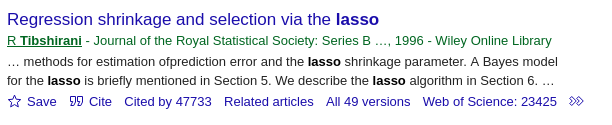
\includegraphics[width=0.8\linewidth]{lasso_citations}
        \caption{This paper on a method for sparse regression has 40,000 citations.}%
    \end{figure}
\end{frame}
\begin{frame}
    What will be new about this method?
    \begin{itemize}
        \item Fast and effective.
        \item Connections to other areas in modern linear algebra.
        \item Works for sparse linear regression and sparse PCA.
        \item Potential to be sped up in future work.
    \end{itemize}
\end{frame}

\begin{frame}
    \begin{figure}[h]
        \centering
        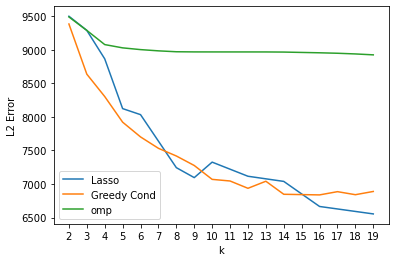
\includegraphics[width=0.8\linewidth]{superconductivity.png}
        \caption{Superconductivity. 81 Columns, 0.03 seconds at the maximum.}%
        \label{fig:superconductivity}
    \end{figure}
\end{frame}
\begin{frame}
    \begin{figure}[h]
        \centering
        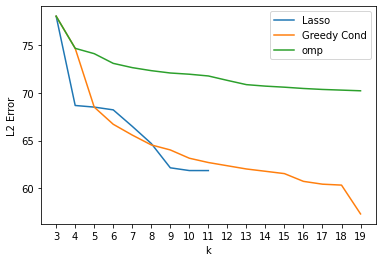
\includegraphics[width=0.8\linewidth]{violentcrime.png}
        \caption{Communities. 101 columns. Under 0.03 seconds at the maximum.}%
        \label{fig:name}
    \end{figure}
\end{frame}
\begin{frame}
    \tiny{
\begin{table}[H]
\begin{center}
    \begin{tabular}{c|c c c c c c}
        Dataset & Columns & $k$ & Found Value & Optimal Value & Gap & Time (s)\\
        \hline
        Wine & 13 & 5 & 3.43 & 3.43 & $<10^{-5}$ & $3\times 10^{-4}$\\
             &    & 10 & 4.45 & 4.59 & $0.03$ & $8\times 10^{-4}$\\
        \hline
        Pitprops & 13 & 5 & 3.40 & 3.40 & $<10^{-5}$ & $3\times 10^{-4}$\\
             &    & 10 & 3.95 & 4.17 & $0.05$ & $8\times 10^{-4}$\\
        \hline
        MiniBooNE & 50 & 5 & 4.99 & 5.00 & $<10^{-5}$ & 0.003\\
             &    & 10 & 9.99 & 9.99 & $<10^{-5}$ & 0.012\\
        \hline
        Communities & 101 & 5 & 4.51 & 4.86 & 0.07 & 0.02 \\
             &    & 10 & 8.71 & 8.82 & $0.013$ & 0.09\\
        \hline
        Arrythmia & 274 & 5 & 4.18 & 4.23 & 0.012 & 0.39\\
         & & 10 & 7.49 & 7.53 & 0.005 & 1.44
    \end{tabular}

\end{center}
\caption{A table describing the results of running an implementation of \Cref{alg:greedy} for sparse PCA on various datasets and values of $k$.  The gap is defined to be $\frac{\text{Optimal Value} - \text{Found Value}}{\text{Optimal Value}}$.}
\end{table}}
\end{frame}
\begin{frame}
    \centering
    \huge
    {\color{gray}Bounds based on Polynomial Roots}
\end{frame}
\begin{frame}
    \frametitle{Motivation}
    \textbf{The following are the same.}
    \vspace{0.3in}
    \begin{columns}
        \begin{column}{0.48\textwidth}
            \begin{block}{Variational Characterization}
            \begin{equation*}
                \begin{aligned}
                    \max\quad & x^{\intercal}Ax\\
                    \st & x^{\intercal}x = 1\\
                \end{aligned}
            \end{equation*}
            \end{block}
        \end{column}
        \begin{column}{0.48\textwidth}
            \begin{block}{Characteristic Polynomial}
            \[
                \max \{t : \det(tI - A) = 0\}.
            \]
            \end{block}
        \end{column}
    \end{columns}
\end{frame}
\begin{frame}
    \frametitle{Motivation}
    Whenever $A_1$ is PSD,
    \vspace{0.3in}
    \begin{columns}
        \begin{column}{0.48\textwidth}
            \begin{block}{QCQP}
            \begin{equation*}
                \begin{aligned}
                    \max\quad & x^{\intercal}A_0x\\
                    \st & x^{\intercal}A_1x = 1\\
                \end{aligned}
            \end{equation*}
            \end{block}
        \end{column}
        \begin{column}{0.48\textwidth}
            \begin{block}{Root}
            \[
                \max \{t : \det(tA_1 - A_0) = 0\}.
            \]
            \end{block}
        \end{column}
    \end{columns}
\end{frame}
\begin{frame}
    \frametitle{Sparse Determinants}
    A \emph{linear combination of minors} polynomial of degree $k$ is a polynomial in a symmetric matrix of indeterminants so that
    \[
        p(X) = \sum_{S \subseteq [n] : |S| = k}a_S\det(X|_S),
    \]
    Here $X|_S$ is the principal submatrix of $X$ indexed by the elements of $S$.
\end{frame}
\begin{frame}
    \frametitle{Sparse Determinants}
    \textbf{Idea:} $\max \{t : \det(tA_1|_S - A_0|_S) = 0\}$ is the value of the program
    \begin{equation*}
        \begin{aligned}
            \max\quad & x^{\intercal}A_0x\\
            \st & x^{\intercal}A_1x = 1\\
                &x \in \R^S
        \end{aligned}
    \end{equation*}
    We want to find the maximum out of all of these roots.
\end{frame}
\begin{frame}
    \frametitle{Sparse Determinants}
    \begin{figure}[h]
        \centering
        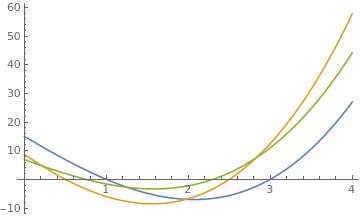
\includegraphics[width=0.6\linewidth]{univariates.png}
        \caption{Each subset of the columns has an associated polynomial.}%
        \label{fig:variety}
    \end{figure}
\end{frame}
\begin{frame}
    \frametitle{Sparse Determinants}
    \begin{figure}[h]
        \centering
        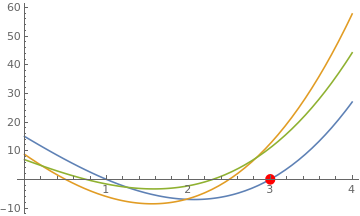
\includegraphics[width=0.6\linewidth]{univariates_root.png}
        \caption{We want the largest out of all of these roots.}%
        \label{fig:variety}
    \end{figure}
\end{frame}
\begin{frame}
    \frametitle{Sparse Determinants}
    \begin{figure}[h]
        \centering
        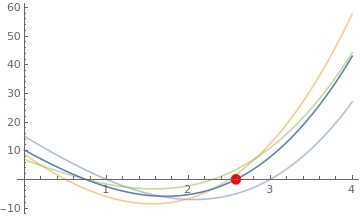
\includegraphics[width=0.6\linewidth]{univariates_average_root.png}
        \caption{Instead, take the average of all of these polynomials and find the maximum root of that.}%
        \label{fig:variety}
    \end{figure}
\end{frame}
\begin{frame}
    \frametitle{An Inequality}
    \begin{block}{Theorem}
        Let $p$ be an LPM polynomial with nonnegative coefficients.  If $A_1$ is PSD, then
        \begin{equation*}
            \begin{aligned}
                \max\quad & x^{\intercal}A_0x\\
                \st & x^{\intercal}A_1x = 1\\
                    &|\supp(x)| \le k.
            \end{aligned}
        \end{equation*}
        is at least 
        \[
            \eta = \max \{y : p(A_1y-A_0) = 0 \}.
        \]
    \end{block}
\end{frame}
\begin{frame}
    \frametitle{An Inequality}
    \begin{block}{Proof}
        Suppose that $p(A_1 \eta-A_0) = 0$, then there must be some $S$ so that 
        \[
            \det(\eta A_1|_S - A_0|_S) \le 0.
        \]
        This means that the maximum root of this polynomial must be at least $\eta$, so that the corresponding optimization problem has a solution that is at least $\eta$.
    \end{block}
\end{frame}
\begin{frame}
    \centering
    \huge
    {\color{gray}A Concrete Version For Sparse Regression}
\end{frame}
\begin{frame}
    \frametitle{Example}
    Sparse regression is a sparse QCQP where
    \[
        A_0 = \hat{b}\hat{b}^{\intercal},
    \]
    \[
        A_1 = A^{\intercal}A,
    \]
    where $\hat{b} = A^{\intercal}b$.
\end{frame}
\begin{frame}
    \frametitle{Example}
    Plugging this into our expression for sparse linear regression, we want to compute
    \[
        \eta = \max \{y : c_n^k(A^{\intercal}Ay-\hat{b}\hat{b}^{\intercal}) = 0 \}.
    \]
    Notice that when $y = 0$, this is $c_n^k(A^{\intercal}Ay-\hat{b}\hat{b}^{\intercal})$, because $\hat{b}\hat{b}^{\intercal}$ is rank 1.

    \pause
    In fact, when $y=0$, this vanishes with multiplicity $k-1$! The polynomial actually must have the form
    \[
        c_n^k(A^{\intercal}Ay-\hat{b}\hat{b}^{\intercal}) = y^{d-1}(k_1y+k_2),
    \]
    for some constants $k_1$ and $k_2$.

\end{frame}
\begin{frame}
    \frametitle{Example}
    \begin{block}{An explicit formula for linear regression}
        \[
            \eta = \frac{c_n^k(A^{\intercal}A+\hat{b}\hat{b}^{\intercal})}{c_n^k(A^{\intercal}A)} - 1.
        \]
    \end{block}
\end{frame}
\begin{frame}
    \frametitle{Example}
    Sanity check: when $k = n$, this becomes
    \[
        \eta = \frac{\det(A^{\intercal}A+\hat{b}\hat{b}^{\intercal})}{\det(A^{\intercal}A)} - 1.
    \]
    \pause
    This turns out to be exactly the formula for the optimal error in ordinary least squares regression, and can be seen as a version of Cramer's rule for solving a system of linear equations.
\end{frame}
\begin{frame}
    \frametitle{A Probabilistic Interpretation}
    \pause
    Let $p(X) = \sum_{S \subseteq [n] : |S| = k} a_S\det(X|_S)$ be LPM.
    
    \pause
    Consider $\pi(S) \alpha a_S\det(AA^{\intercal}|_S)$ be the law of a \emph{weighted determinantal point process}. This selects a random subset of $[n]$ proportional to the determinant of $\det(AA^{\intercal}|_S)$. Then,
    \[
        \eta = \E[\ell(A_S, b)],
    \]
    where $\ell(A, b) = \min \{\|Ax - b\|^2\}$.
\end{frame}

\begin{frame}
    \centering
    \huge
    {\color{gray}Applications of this Inequality}
\end{frame}
\begin{frame}
    \frametitle{An Inequality}
    \begin{block}{Theorem}
        Let $p$ be an LPM polynomial with nonnegative coefficients.  If $A_1$ is PSD, then
        \begin{equation*}
            \begin{aligned}
                \max\quad & x^{\intercal}A_0x\\
                \st & x^{\intercal}A_1x = 1\\
                    &|\supp(x)| \le k.
            \end{aligned}
        \end{equation*}
        is at least 
        \[
            \eta = \max \{y : p(A_1y-A_0) = 0 \}.
        \]
    \end{block}
\end{frame}
\begin{frame}
    \frametitle{What do we do with this inequality?}
    Two questions:
    \begin{itemize}
        \item Are there LPM polynomials that we can find the roots of quickly?
        \pause 
        \item Can we efficiently find a solution to the sparse QCQP that does at least as well as this result guarantees?
        \pause
        \item Is this inequality any good?
    \end{itemize}
\end{frame}
\begin{frame}
    \frametitle{What now?}
    Two questions:
    \begin{itemize}
        \item \textbf{Are there LPM polynomials that we can find the roots of quickly?}
        \item Can we efficiently find a solution to the sparse QCQP that does at least as well as this result guarantees?
        \item Is this inequality any good?
    \end{itemize}
\end{frame}
\begin{frame}
    \frametitle{Characteristic Coefficients}
    Define
    \[
        c_n^k(Y) = \sum_{\top{S \subseteq [n]}{|S| = k}}  \det(Y|_S).
    \]
    \pause 
    This is an LPM polynomial with very simple coefficients.
\end{frame}
\begin{frame}
    \frametitle{Characteristic Coefficients}
    \begin{block}{Facts About Characteristic Coefficients}
        $c_n^k(Y)$ is sometimes called a \emph{characteristic coefficient}, since it is a coefficient of the characteristic polynomial of $Y$, i.e.
        \[
            \det(Y + tI) = \sum_{j=0}^n c_n^{n-j}(Y) t^j.
        \]
        \pause
        In particular, it is
        \begin{itemize}
            \item Basis invariant, so that $c_n^k(U^{\intercal} Y U) = c_n^k(Y)$ for any orthogonal matrix $U$.
            \pause
            \item Efficiently computable.
            \pause
            \item For $Y$ in the interior of $S^k_n$, $c_n^k(Y) > 0$.
            \pause
            \item If $X$ is PSD, then $c_n^k(tX+Y)$ has only real roots for any $Y$.
        \end{itemize}
    \end{block}
\end{frame}
\begin{frame}
    \frametitle{Newton's Method for Real Rooted Polynomials}
    \begin{block}{Theorem}
        If $p(t)$ is a real rooted polynomial of degree $d$, then for large enough $t_0$, Newton's method converges to the maximum root of $p(t)$ in $O(d \log(t_0 / \epsilon))$ steps.
    \end{block}
    Interpolation let's me evaluate $p(t)$ at $d$ points, then apply Newton's method.
\end{frame}
\begin{frame}
    \frametitle{What now?}
    Two questions:
    \begin{itemize}
        \item Are there LPM polynomials that we can find the roots of quickly?
            \begin{itemize}
                \item Yes!
            \end{itemize}
        \item Can we efficiently find a solution to the sparse QCQP that does at least as well as this result guarantees?
        \item Is this inequality any good?
    \end{itemize}
\end{frame}
\begin{frame}
    \frametitle{What now?}
    Two questions:
    \begin{itemize}
        \item Are there LPM polynomials that we can find the roots of quickly?
            \begin{itemize}
                \item Yes!
            \end{itemize}
        \item Can we efficiently find a solution to the sparse QCQP that does at least as well as this result guarantees?
            \begin{itemize}
                \item Yes!
            \end{itemize}
        \item Is this inequality any good?
            \begin{itemize}
                \item Not really, but this can be fixed.
            \end{itemize}
    \end{itemize}
    \pause
    Both of these will be resolved by introducing different coefficients.
\end{frame}
\begin{frame}
    \centering
    \huge
    {\color{gray}Conditioning}
\end{frame}
\begin{frame}
    \frametitle{Introducing Coefficients}
    Recall
    \[
        c_n^k(Y) = \sum_{\top{S \subseteq [n]}{|S| = k}}  \det(Y|_S).
    \]
    \pause 
    This averages over all supports of size $k$. We want to find a single support set.
\end{frame}
\begin{frame}
    \frametitle{Conditioning}
    \textbf{Idea:} Reduce the size of the support of $p$.
    For a LPM polynomial $p$, and $i \in [n]$, define the conditioning.
    \[
        p|_i = \sum_{S : i \in S} a_S \det(X|_S).
    \]
    This has support strictly smaller than $p$. Is it better than $p$?
\end{frame}
\begin{frame}
    \frametitle{Conditioning}
    \begin{theorem}
    For any LPM polynomial $p$ with nonnegative coefficients, there exists some $i$ so that
    \[
        \eta_{p|_i} \ge \eta_{p}.
    \]
    \end{theorem}
\end{frame}
\begin{frame}
    \frametitle{Conditioning}
    Consider
        \begin{align*} 
        \sum_{i \in [n]} p|_{i}&=\sum_{i \in [n]} \sum_{i \in  S} a_S \det(X|_S)\\
                &=k\sum_{S} a_S \det(X|_S)\\
                &=kp
        \end{align*}
\end{frame}
\begin{frame}
    \frametitle{Conditioning}
    \[
        \sum_{i\in [n]}p|_i(\eta_p) = kp(\eta_p) = 0.
    \]
    \pause
    Therefore, for some $i$, $ p|_{i}(\eta_{p}) \le 0$.
    \pause
    This implies that the largest root of $p|_{i}$ is at least $\eta_{p}$.
\end{frame}
\begin{frame}
    \frametitle{Conditioning and Determinantal Point Processes}
    Recall that if we are working with sparse regression, for any LPM polynomial $p$,
    \[
        \eta_p = \E[\ell(A_S, b)],
    \]
    where the expectation is taken with respect to some weighted DPP.

    Then,
    \[
        \eta_{p|_i} = \E[\ell(A_S, b)|i \in S],
    \]
\end{frame}
\begin{frame}
    \frametitle{Computing Conditionings}
    We want to compute
    \[
        p|_i = \sum_{S : i \in S} a_S \det(X|_S).
    \]
    How can we do this?
\end{frame}
\begin{frame}
    \frametitle{Computing Conditionings}
    \emph{Idea: } Notice that
    \begin{align*}
        \frac{\partial}{\partial X_{ii}} p(X) &= \sum_{S} a_S \partial_{X_{ii}} \det(X|_{S})\\
                               &= \sum_{S : i \in S} a_S \det(X|_{S \setminus i})
    \end{align*}
\end{frame}
\begin{frame}
    \frametitle{Computing Conditionings}
    Also, recall the Schur complement identity for determinants:
    \begin{align*}
        \det(X) = X_{ii} \det(X \setminus i),
    \end{align*}
    where 
    \[
        X \setminus i = X - \frac{1}{X_{ii}} X_i X_i^{\intercal}.
    \]
    Here, $X_i$ is the $i^{th}$ column of $X$.
\end{frame}
\begin{frame}
    \frametitle{Computing Conditionings}
    Putting these together,
    \[
        p|_i(X) = X_{ii} \frac{\partial}{\partial X_{ii}} p(X \setminus i).
    \]
    When $p = c_n^k$, $\frac{\partial}{\partial X_{ii}} p(X) = c_{n-1}^{k-1}(X)$, so 
    \[
        p|_i(X) = X_{ii} c_{n-1}^{k-1}(X \setminus i).
    \]
\end{frame}
\begin{frame}
    \frametitle{Computing Conditionings}
    It's also true that if $p$ is LPM and $p(A_1 t - A_0)$ has real roots for all PSD $A_1$, then the same is true for $p|_i$.
\end{frame}
\begin{frame}
    \centering
    \huge
    {\color{gray}Algorithms}
\end{frame}
\begin{frame}
    \frametitle{An Algorithm for Sparse QCQPs}
    Putting it all together,
    \begin{algorithm}[H]
    \caption{The Greedy Conditioning Heuristic}
    \label{alg:greedy}
    \begin{algorithmic}
        \State $T \gets \varnothing$
        \For{$t = 1 \dots k$}
            \State $j \gets \argmax \eta_{p|_{T + j}}$
            \State $T \gets T + j$
        \EndFor

        \Return $T$
    \end{algorithmic}
    \end{algorithm}

    We have seen that this will always produce an answer which is at least $\eta_p$, and we have means of computing all of these things efficiently.
\end{frame}
\begin{frame}
    \frametitle{An Algorithm for Sparse QCQPs}
    This already gives the accuracy competitive with LASSO and others that we saw at the beginning of the talk, but computing everything naively is slow (1000x slower than LASSO)!

    \pause
    We can speed it up by a lot by doing incremental computations: instead of recomputing characteristic coefficients, we will use efficient update formulas and diagonalization maintance.
\end{frame}
\begin{frame}
    \frametitle{Computing Characteristic Polynomials.}
    Let $X = QDQ^{\intercal}$ be the diagonalization of a matrix $X$, i.e.
    \begin{itemize}
        \item $Q$ is the orthogonal matrix whose columns are eigenvectors of $X$.
        \item $D$ is diagonal and its entries are eigenvalues of $X$.
    \end{itemize}
\end{frame}
\begin{frame}
    \frametitle{Computing Characteristic Polynomials.}
    $c_n^k(X)$ is given by the elementary symmetric polynomial in the eigenvalues of $X$:
    \[
        c_n^k(X) = \sum_{S \subseteq [n],|S| = k} \prod_{i \in S}\lambda_i,
    \]
    where the $\lambda_i$ are eigenvalues of $X$.
\end{frame}
\begin{frame}
    \frametitle{Computing Characteristic Polynomials.}
    If the diagonalization of $X$ is given, the characteristic coefficient can be computed in $O(nk)$ time using dynamic programming to compute the elementary symmetric polynomial in the eigenvalues.
\end{frame}
\begin{frame}
    \frametitle{Computing Characteristic Polynomials.}
    Now, what if we want to compute
    \[
        p|_i(X) = X_{ii} c_{n-1}^{k-1}(X - \frac{1}{X_{ii}X_iX_i^{\intercal})?
    \]
    \textbf{Idea: } Use rank 1 updates instead of recomputing.
\end{frame}
\begin{frame}
    \frametitle{Computing Characteristic Polynomials.}
    Because $\frac{1}{X_{ii}X_iX_i^{\intercal}$ is rank 1, the first order Taylor expansion gives an exact answer:
    \[
        c_{n-1}^{k-1}(X - \frac{1}{X_{ii}X_iX_i^{\intercal}) = c_{n-1}^{k-1}(X)  - \frac{1}{X_{ii}X_i^{\intercal}\nabla c_{n-1}^{k-1}(X)X_i.
    \]
    If we already have $c_{n-1}^{k-1}(X)$ for each $i$, we really just want to compute
    \[
        X_i^{\intercal}\nabla c_{n-1}^{k-1}(X)X_i.
    \]
\end{frame}
\begin{frame}
    \frametitle{Computing Characteristic Polynomials.}
    \textbf{Idea:} We can change basis because characteristic coefficients are basis invariant, so
    \[
        X_i^{\intercal}\nabla c_{n-1}^{k-1}(X)X_i = 
        Q_i^{\intercal}D\nabla c_{n-1}^{k-1}(D)DQ_i,
    \]
    where $Q_i$ is the $i^{th}$ row of $Q$.
\end{frame}

%\begin{frame}
%    \centering
%    \huge
%    {\color{gray}A Warm Up}
%\end{frame}
%\begin{frame}
%\frametitle{Semidefinite Programming Relaxations}
%    For non-sparse QCQPs, there is a standard Schur relaxation, which is a convex
%    optimization problem.
%    \begin{equation*}
%        \begin{aligned}
%            \max\quad & x^{\intercal}Ax\\
%            \st & x^{\intercal}x = 1\\
%        \end{aligned}
%    \end{equation*}
%    \vspace{0.6in}
%\end{frame}
%\begin{frame}
%\frametitle{Semidefinite Programming Relaxations}
%    For non-sparse QCQPs, there is a standard Schur relaxation, which is a convex
%    optimization problem.
%    \begin{equation*}
%        \begin{aligned}
%            \max\quad & \tr(Axx^{\intercal})\\
%            \st & \tr(xx^{\intercal}) = 1\\
%        \end{aligned}
%    \end{equation*}
%    \vspace{0.6in}
%\end{frame}
%\begin{frame}
%\frametitle{Semidefinite Programming Relaxations}
%    For non-sparse QCQPs, there is a standard Schur relaxation, which is a convex
%    optimization problem.
%    \begin{equation*}
%        \begin{aligned}
%            \max\quad & \tr(AX)\\
%            \st & \tr(X) = 1\\
%            & X = xx^{\intercal}
%        \end{aligned}
%    \end{equation*}
%    \vspace{0.3in}
%\end{frame}
%\begin{frame}
%\frametitle{Semidefinite Programming Relaxations}
%    For non-sparse QCQPs, there is a standard Schur relaxation, which is a convex
%    optimization problem.
%    \begin{equation*}
%        \begin{aligned}
%            \max\quad & \tr(AX)\\
%            \st & \tr(X) = 1\\
%                & X \in S_n\\
%        \end{aligned}
%    \end{equation*}
%    \pause 
%    \[
%        S_n = \conv \{ xx^{\intercal} : x \in \R^n\} = \{X : X \succeq 0\}
%    \]
%\end{frame}
%\begin{frame}
%\frametitle{Semidefinite Programming Relaxations}
%    For a convex cone, $C$, we define the dual 
%    \[
%        C^* = \{y : \forall x \in C,\;\langle y, x \rangle \ge 0 \}.
%    \]
%
%
%    For $S_n$,
%    \[
%        S_n^* = S_n.
%    \]
%\end{frame}
%\begin{frame}
%\frametitle{Semidefinite Programming Relaxations}
%    Every convex optimization problem of this form has a dual, which has the same value (as long as the problem satisfies a certain technical condition).
%    \hspace{0.3in}
%    \begin{columns}
%        \begin{column}{0.5\textwidth}
%            \begin{equation*}
%                \begin{aligned}
%                    \max\quad & \tr(AX)\\
%                    \st & \tr(X) = 1\\
%                        & X \in S_n\\
%                \end{aligned}
%            \end{equation*}
%        \end{column}
%        \begin{column}{0.5\textwidth}
%            \begin{equation*}
%                \begin{aligned}
%                    \min\quad & y\\
%                    \st & Iy - A \in S_n^*\\
%                \end{aligned}
%            \end{equation*}
%        \end{column}
%    \end{columns}
%\end{frame}
%\begin{frame}
%\frametitle{Semidefinite Programming Relaxations}
%    So, we are left with
%    \begin{equation*}
%        \begin{aligned}
%            \min\quad & y\\
%            \st & Iy - A \in S_n^*\\
%        \end{aligned}
%    \end{equation*}
%    How do we solve this?
%\end{frame}
%\begin{frame}
%\frametitle{Semidefinite Programming Relaxations}
%    \begin{document}
%    \tikzset{
%  mynode/.style={fill,circle,inner sep=2pt,outer sep=0pt}
%}
%    \begin{figure}
%        \centering
%          \begin{tikzpicture}
%            \draw[black,thick] (0,0) -- (7,0);
%            \draw[green,thick] (3,0) -- (5,0)
%                node[pos=0,mynode,fill=red,label=above:\textcolor{red}{$y^*$}]{}
%                node[pos=1,mynode,fill=blue,text=blue,label=above:\textcolor{blue}{}]{};
%          \end{tikzpicture}
%    \end{figure}
%    \end{document}
%\end{frame}
%\begin{frame}
%\frametitle{Semidefinite Programming Relaxations}
%    \begin{block}{Fact}
%        $X \in S_n$ if and only if $\det(X|_S) \ge 0$ for all $S \subseteq [n]$. $X \in \partial  S_n$ if and only if $\det(X) = 0$.
%    \end{block}
%\end{frame}
%\begin{frame}
%\frametitle{Semidefinite Programming Relaxations}
%For $y^*$ to be optimal, it must lie on the boundary of $\{y : Iy - A \succeq 0\}$, so $\det(Iy^*-A) = 0$.
%
%Finally, all $t$ large enough, $Iy - A \in S_n$, so the solution to this optimization problem is
%\[
%    \max \{y : \det(Iy - A) = 0\}.
%\]
%
%\end{frame}
%\begin{frame}
%    \frametitle{Summary}
%    \vspace{0.3in}
%    \begin{columns}
%        \begin{column}{0.48\textwidth}
%            \begin{block}{Variational Characterization}
%            \begin{equation*}
%                \begin{aligned}
%                    \max\quad & x^{\intercal}Ax\\
%                    \st & x^{\intercal}x = 1\\
%                \end{aligned}
%            \end{equation*}
%            \end{block}
%        \end{column}
%        \begin{column}{0.48\textwidth}
%            \begin{block}{Characteristic Polynomial}
%            \[
%                \max \{t : \det(tI - A) = 0\}.
%            \]
%            \end{block}
%        \end{column}
%    \end{columns}
%    \textbf{These are equal because $\det(\cdot)$ is a barrier function for the dual cone.}
%\end{frame}
\begin{frame}
    \centering
    \huge
    {\color{gray}A Convex Formulation for Sparse QCQPs}
\end{frame}
\begin{frame}
\frametitle{Semidefinite Programming Relaxations for Sparse QCQPs}
    \begin{equation*}
        \begin{aligned}
            \max\quad & x^{\intercal}A_0x\\
            \st & x^{\intercal}A_1x = 1\\
                &|\supp(x)| \le k
        \end{aligned}
    \end{equation*}

    We can reformulate sparse QCQPs into a convex optimization problem, in a way that is analogous to the standard SDP relaxation of a QCQP.
\end{frame}
\begin{frame}
\frametitle{Semidefinite Programming Relaxations for Sparse QCQPs}
    \begin{equation*}
        \begin{aligned}
            \max\quad & \tr(A_0X)\\
            \st & \tr(A_1X) = 1\\
                & X = xx^{\intercal}\\
                &|\supp(x)| \le k
        \end{aligned}
    \end{equation*}

    Linearize this problem by introducing a new symmetric matrix variable $X$, representing $xx^{\intercal}$.
\end{frame}
\begin{frame}
\frametitle{Semidefinite Programming Relaxations for Sparse QCQPs}

    \begin{equation*}
        \begin{aligned}
            \max\quad & \tr(A_0X)\\
            \st & \tr(A_1X) = 1\\
                & {\color{red}X = xx^{\intercal}}\\
                & {\color{red} |\supp(x)| \le k}
        \end{aligned}
    \end{equation*}

    Linearize this problem by introducing a new symmetric matrix variable $X$, representing $xx^{\intercal}$.
\end{frame}
\begin{frame}
\frametitle{Semidefinite Programming Relaxations for Sparse QCQPs}
    For \emph{sparse} QCQPs, we can consider a sparse version of an SDP:
    \begin{equation*}
        \begin{aligned}
            \max\quad & \tr(A_0X)\\
            \st & \tr(A_1X) = 1\\
                & {\color{red}X \in \FW^k_n}\\
        \end{aligned}
    \end{equation*}
    \pause 
    \[
        \FW^k_n = \conv \{xx^{\intercal} : x\in \R^n,\;|\supp(x)| \le k\} \subseteq \Sym. 
    \]
\end{frame}
\begin{frame}
    \frametitle{Duality}
    There is a conical dual to $\FW^k_n$:
    \[
        S^k_n = \{Y \in \Sym : \forall S : |S| = k, \;Y|_S \succeq 0\}.
    \]
\end{frame}
\begin{frame}
    \frametitle{Duality}
    For most values of $A_1$, the following are equivalent:
    \begin{columns}
        \begin{column}{0.5\textwidth}
            \begin{equation*}
                \begin{aligned}
                    \max\quad & \tr(A_0X)\\
                    \st & \tr(A_1X) = 1\\
                        & X \in \FW^k_n\\
                \end{aligned}
            \end{equation*}
        \end{column}
        \begin{column}{0.5\textwidth}
            \begin{equation*}
                \begin{aligned}
                    \min\quad & y\\
                    \st & A_1y - A_0 \in S^k_n\\
                \end{aligned}
            \end{equation*}
        \end{column}
    \end{columns}
\end{frame}
\begin{frame}
    \frametitle{Duality}
    In words, $S^k_n$ are those symmetric matrices where all of their $k\times k$ minors are PSD.
    \begin{itemize}
        \item ``Local'' version of the PSD cone.
        \item Captures the difficulty of sparse QCQPs.
    \end{itemize}
\end{frame}
\begin{frame}
    \frametitle{$S^k_n$}
    \begin{block}{Fact}
        $X \succeq 0$ if and only if $\det(X|_S) \ge 0$ for all $S \subseteq [n]$.
    \end{block}
\end{frame}
\begin{frame}
    \frametitle{$S^k_n$}
    \begin{block}{Corollary}
        $Y \in S^k_n$ if and only if

        \hspace{0.25in} \emph{for any $S \subseteq [n]$ with $|S| \le k$, $\det(Y|_S) \ge 0$.}
    \end{block}

    A matrix is in $S^k_n$ if and only if all \emph{sufficiently small} submatrices have nonnegative determinant.
\end{frame}
\begin{frame}
    \frametitle{Characteristic Coefficients}
    \begin{block}{Defining the Hyperbolicity Cone}
        Define the \emph{zero-free region of $\Sym$} to be 
        \[
            F(c^k_n) = \{ X \in \Sym : c_n^k(X) \neq 0\}.
        \]
    \end{block}
\end{frame}
\begin{frame}
    \frametitle{Characteristic Coefficients}
    \begin{block}{Defining the Hyperbolicity Cone}
        Define the \emph{hyperbolicity cone} to be 
        \[
            H(c^k_n) = \text{The connected component of }F(c^k_n) \text{ containing }I.
        \]
    \end{block}
\end{frame}
\begin{frame}
    \frametitle{$S^k_n$}
    \begin{figure}[h]
        \centering
        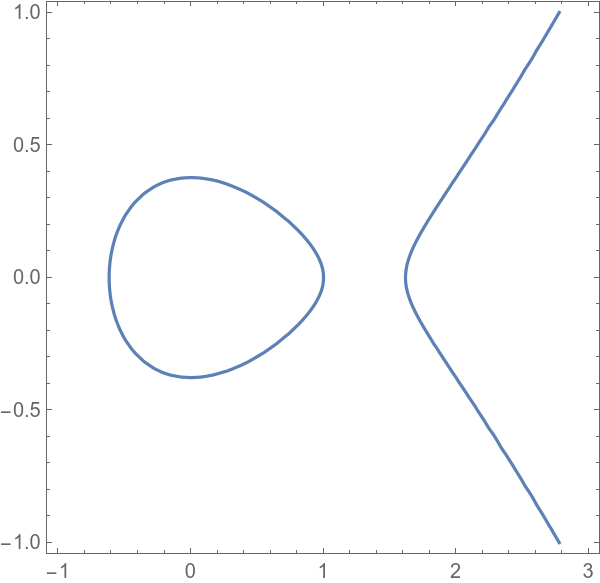
\includegraphics[width=0.6\linewidth]{variety.png}
        \caption{A cartoon of $F(c^k_n)$}%
        \label{fig:variety}
    \end{figure}
\end{frame}
\begin{frame}
    \frametitle{$S^k_n$}
    \begin{figure}[h]
        \centering
        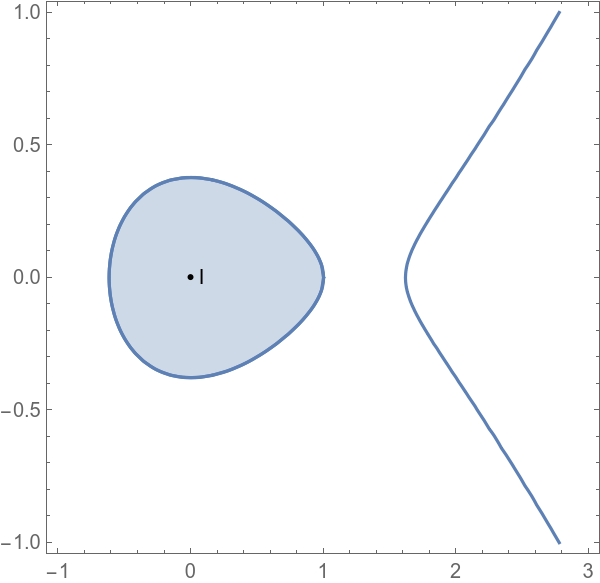
\includegraphics[width=0.6\linewidth]{hcone.png}
        \caption{A cartoon of $H(c^k_n)$}%
        \label{fig:variety}
    \end{figure}
\end{frame}
\begin{frame}
    \frametitle{$S^k_n$}
    $H(c^k_n)$.
    \begin{itemize}
        \item Basis invariant, so that $U^{\intercal} Y U \in H(c^k_n)$ if and only if $Y \in H(c^k_n)$ for any orthogonal matrix $U$.
        \pause
        \item Efficiently computable.
        \pause
        \item $S^k_n \subseteq H(c^k_n).$
        \pause
        \item Convex, which follows from the theory of \emph{hyperbolic polynomials}. It is called the \emph{hyperbolicity cone} associated with the polynomial $c_n^k$.
    \end{itemize}
\end{frame}
\begin{frame}
    \frametitle{A Picture of the Relaxation}
    \begin{figure}[h]
        \centering
        
\includegraphics[width=0.6\linewidth]{just_snk.png}
        \caption{$S^{k}_n$}%
        \label{fig:just_snk}
    \end{figure}
\end{frame}
\begin{frame}
    \frametitle{A Picture of the Relaxation}
    \begin{figure}[h]
        \centering
        
\includegraphics[width=0.6\linewidth]{comparison.png}
        \caption{$S^{k}_n$ and $H(c^k_n)$}%
        \label{fig:just_snk}
    \end{figure}
\end{frame}
\begin{frame}
    \frametitle{Applications}
    \begin{itemize}
        \item Eigenvalues of Matrices in $S^k_n$.
        \item An algorithm for Sparse QCQPs.
    \end{itemize}
\end{frame}
\begin{frame}
    \centering
    \huge
    {\color{gray}Eigenvalues of Matrices in $S^k_n$.}
\end{frame}
\begin{frame}
    \frametitle{Distances}
    \begin{block}{Question}
        Let $Y \in S^k_n$. How far away can $Y$ be from being PSD?
    \end{block}
    \pause
    \begin{block}{Formal Question}
        Let $Y \in S^k_n$, and $\tr(Y)=1$. How small can $\lambda_{min}(Y)$ be?
    \end{block}
\end{frame}
\begin{frame}
    \frametitle{Eigenvalues in $S^k_n$}
    \begin{equation*}
        \begin{aligned}
            \min\quad & \lambda_{min}(Y)\\
            \st & \tr(Y) = 1\\
                & Y \in S^k_n\\
        \end{aligned}
    \end{equation*}
    \pause
    \begin{itemize}
        \item A basic linear algebra question?
        \pause
        \item Concave minimization (hard).
        \pause
        \item Complicated objective.
    \end{itemize}
\end{frame}
\begin{frame}
    \frametitle{Eigenvalues in $S^k_n$}
    Relax the following program
    \begin{equation*}
        \begin{aligned}
            \min\quad & \lambda_{min}(Y)\\
            \st & \tr(Y) = 1\\
                & Y \in S^k_n\\
        \end{aligned}
    \end{equation*}
\end{frame}
\begin{frame}
    \frametitle{Eigenvalues in $S^k_n$}
    Relax the following program
    \begin{equation*}
        \begin{aligned}
            \min\quad & \lambda_{min}(Y)\\
            \st & \tr(Y) = 1\\
                & Y \in {\color{red}H(c_n^k)}\\
        \end{aligned}
    \end{equation*}
\end{frame}
\begin{frame}
    \frametitle{Eigenvalues in $S^k_n$}
    Apply basis invariance
    \begin{equation*}
        \begin{aligned}
            \min\quad & \lambda_{min}(Y)\\
            \st & \tr(Y) = 1\\
                & {\color{red}Y \text{ is diagonal}}\\
                & Y \in H(c_n^k)
        \end{aligned}
    \end{equation*}
\end{frame}
\begin{frame}
    \frametitle{Eigenvalues in $S^k_n$}
    Apply permutation invariance.
    \begin{equation*}
        \begin{aligned}
            \min\quad & {\color{red}Y_{11}}\\
            \st & \tr(Y) = 1\\
                & Y \text{ is diagonal}\\
                & Y \in H(c_n^k)
        \end{aligned}
    \end{equation*}
\end{frame}
\begin{frame}
    \frametitle{Eigenvalues in $S^k_n$}
    \begin{equation*}
        \begin{aligned}
            \min\quad & Y_{11}\\
            \st & \tr(Y) = 1\\
                & Y \text{ is diagonal}\\
                & Y \in H(c_n^k)
        \end{aligned}
    \end{equation*}
    \pause
    These last 3 constraints are permutation invariant, so by convexity, this reduces to a 1-dimensional optimization problem!

    The minimum turns out to be 
    \[
        \frac{k-n}{n(k-1)}.
    \]

\end{frame}
\begin{frame}
    \frametitle{Eigenvalues in $S^k_n$}
    This is also the minimum eigenvalue of the matrix
    \[
        G(n,k) = 
        \frac{1}{n}
        \begin{pmatrix}
            1 & -\frac{1}{k-1} & -\frac{1}{k-1}  &\dots& -\frac{1}{k-1}\\
            -\frac{1}{k-1} & 1 & -\frac{1}{k-1}  &\dots& -\frac{1}{k-1}\\
            \dots\\
            -\frac{1}{k-1} & -\frac{1}{k-1}& -\frac{1}{k-1}  &\dots & 1\\
        \end{pmatrix},
    \]
    which is in $S^k_n$.

    This implies that $\frac{k-n}{n(k-1)}$ is precisely the solution to the original optimization problem over $S^k_n$.
\end{frame}
\begin{frame}
    \frametitle{Takeaways}
    \begin{itemize}
        \item We can precisely compute the value of this nonconvex eigenvalue minimization problem.
        \item We can control the set $S^k_n$ (which is useful in sparse optimization) using polynomial functions (which are tractable).
    \end{itemize}
\end{frame}
\begin{frame}
    \frametitle{$S^k_n$}
    \begin{figure}[h]
        \centering
        
\includegraphics[width=0.6\linewidth]{comparison.png}
    \end{figure}
\end{frame}
\begin{frame}
    \frametitle{Stepping Back}
    \begin{figure}[h]
        \centering
        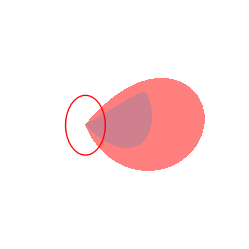
\includegraphics[width=0.6\linewidth]{comparison_circle.png}
        \caption{$S^{n,k}$ and $H$}%
        \label{fig:just_snk}
    \end{figure}
\end{frame}
\begin{frame}
    \centering
    \huge
    {\color{gray}A Heuristic for Sparse QCQPs}
\end{frame}
\begin{frame}
    \frametitle{Hyperbolicity Cones and Sparse QCQPs}
    We can now perform a relaxation
    \begin{equation*}
        \begin{aligned}
            \min\quad & y\\
            \st & A_1y - A_0 \in S^k_n\\
        \end{aligned}
    \end{equation*}
\end{frame}
\begin{frame}
    \frametitle{Hyperbolicity Cones and Sparse QCQPs}
    We can now perform a relaxation
        \begin{equation*}
            \begin{aligned}
                \min\quad & y\\
                \st & A_1y - A_0 \in {\color{red} H(c_n^k)}\\
            \end{aligned}
        \end{equation*}
    \pause
\end{frame}
\begin{frame}
    \frametitle{Hyperbolicity Cones and Sparse QCQPs}
    \frametitle{Stepping Back}
    \begin{figure}[h]
        \centering
        
\includegraphics[width=0.6\linewidth]{comparison.png}
        \caption{$S^{n,k}$ and $H$}%
        \label{fig:just_snk}
    \end{figure}
\end{frame}
\begin{frame}
    \frametitle{Hyperbolicity Cones and Sparse QCQPs}
    \begin{figure}[htpb]
        \centering
        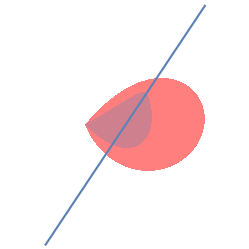
\includegraphics[width=0.6\linewidth]{comparison_line.png}
        \caption{Adding a constraint}%
        \label{fig:comparison_line}
    \end{figure}
\end{frame}
\begin{frame}
    \frametitle{Hyperbolicity Cones and Sparse QCQPs}
    \begin{figure}[htpb]
        \centering
        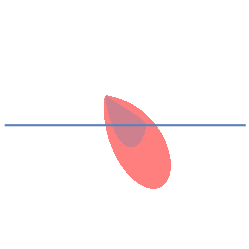
\includegraphics[width=0.6\linewidth]{comparison_line_rotated.png}
        \caption{Adding a constraint}%
        \label{fig:comparison_line}
    \end{figure}
\end{frame}
\begin{frame}
    \frametitle{Hyperbolicity Cones and Sparse QCQPs}
    \begin{figure}[htpb]
        \centering
        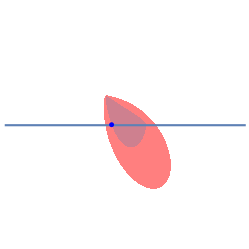
\includegraphics[width=0.6\linewidth]{optimum.png}
        \caption{Optimum we wish to find}%
        \label{fig:comparison_line}
    \end{figure}
\end{frame}
\begin{frame}
    \frametitle{Hyperbolicity Cones and Sparse QCQPs}
    \begin{figure}[htpb]
        \centering
        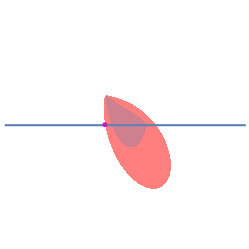
\includegraphics[width=0.6\linewidth]{relaxed.png}
        \caption{Relaxed Value}%
        \label{fig:comparison_line}
    \end{figure}
\end{frame}
\begin{frame}
    \frametitle{Hyperbolicity Cones and Sparse QCQPs}
    \begin{block}{Key Fact}
        \[\partial H(c_n^k) = \{X \in H(c_n^k) : c_n^k(X) = 0\}.\]
    \end{block}
\end{frame}
\begin{frame}
    \frametitle{Hyperbolicity Cones and Sparse QCQPs}
    So, the optimization problem 

    \begin{equation*}
        \begin{aligned}
            \min\quad & y\\
            \st & A_1y - A_0 \in H(c_n^k)\\
        \end{aligned}
    \end{equation*}

    is intimately related to the question, \emph{what are the roots of the univariate polynomial $g(y) = c_n^k(A_1y-A_0)$?}
\end{frame}
\begin{frame}
    \frametitle{Hyperbolicity Cones and Sparse QCQPs}
    \begin{block}{Theorem}
        If $A_1$ is PSD, then 
        \begin{equation*}
            \begin{aligned}
                \min\quad & y\\
                \st & A_1y - A_0 \in H(c_n^k)\\
            \end{aligned}
        \end{equation*}
        is exactly the maximum root of $c_n^k(A_1y-A_0)$.
    \end{block}
\end{frame}
\begin{frame}
    \frametitle{Hyperbolicity Cones and Sparse QCQPs}
    \begin{figure}[htpb]
        \centering
        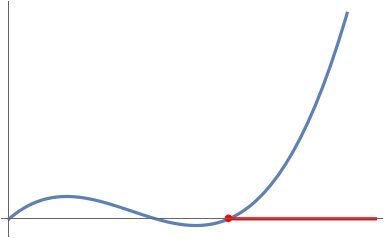
\includegraphics[width=0.8\linewidth]{roots.png}
        \caption{Roots}%
        \label{fig:roots}
    \end{figure}
\end{frame}
\begin{frame}
    \begin{block}{Theorem}
        If $A_1$ is PSD, then
        \begin{equation*}
            \begin{aligned}
                \max\quad & x^{\intercal}A_0x\\
                \st & x^{\intercal}A_1x = 1\\
                    &|\supp(x)| \le k.
            \end{aligned}
        \end{equation*}
        is at least 
        \[
            \eta = \max \{y : c_n^k(A_1y-A_0) = 0 \}.
        \]
    \end{block}
\end{frame}
\begin{frame}
    \frametitle{Example}
    Remember sparse linear regression:
    \begin{equation*}
        \begin{aligned}
        \max\quad & x^{\intercal}A^{\intercal}bb^{\intercal}Ax\\
        \st & x^{\intercal}A^{\intercal}Ax = 1\\
            & |\supp(x)| \le k.
        \end{aligned}
    \end{equation*}
\end{frame}
\begin{frame}
    \centering
    \huge
    {\color{gray}Introducing Coefficients}
\end{frame}
\begin{frame}
    \frametitle{An Algorithm for Sparse QCQPs}
    
This always returns some $T$ so that 
\begin{equation*}
    \begin{aligned}
        \max\quad & x^{\intercal}A_0x\\
        \st & x^{\intercal}A_1x = 1\\
            & \supp(x) = T
    \end{aligned}
\end{equation*}
is at least $\eta_p$.
\end{frame}
\begin{frame}
    \frametitle{How do we efficiently compute $p|_T$?}
    Define the Schur-complement of $X$ with respect to $i \in [n]$ to be
    \[
        X \setminus i = X - X_{i,i}^{-1} X_{i} X_{i}^{\intercal}.
    \]

    Then,
    \begin{align*} 
        (c_n^k)|_i(X)&=X_{i,i} \; c_n^{k-1}(X \setminus i)\\
    \end{align*}
    Because $X \setminus i$ differs from $X$ by a rank 1 matrix, we can use ideas from dynamic algorithms to simultaneously compute this for all $i$ in $O(n^{\omega})$ time.

    For sparse regression, this gives a $O(n^3+kn^{\omega})$ time algorithm for performing the greedy update.
\end{frame}
\begin{frame}
    \centering
    \huge
    {\color{gray}Experimental Results}
\end{frame}

\begin{frame}
    \frametitle{Open Problems}
    \begin{itemize}
        \item Does this really work? Can we prove it?
        \item Can we do more interesting combinatorial constraints on the support?
        \item Can we use these roots in a more clever (or less greedy way)?
    \end{itemize}
\end{frame}
%\begin{frame}
%    \frametitle{Positive Semidefinite Matrices}
%    \begin{block}{Definition}
%        An $n\times n$ symmetric matrix $A$ is PSD if all of its eigenvalues are nonnegative.
%    \end{block}
%
%    {\large \textbf{Equivalent Conditions}}
%    \begin{itemize}
%        \item The quadratic form $q(x) = x^{\intercal}Ax$ is nonnegative for all $x$.
%        \item The determinants of all principal submatrices of $A$ are nonnegative.
%        \item $A$ can be factored as $V^{\intercal}V$.
%        \item There are vectors $v_1 ,\dots, v_n$ so that $A_{ij} = \langle v_i, v_j\rangle$ for each $i$, $j$ in $[n]$.
%    \end{itemize}
%
%\end{frame}
%\begin{frame}
%    \frametitle{Positive Semidefinite Matrices}
%    \begin{figure}[H]
%    \begin{subfigure}{0.5\textwidth}
%        \[
%            \begin{pmatrix}
%                1 & 1 & 1 & 1\\
%                1 & 1 & 1 & 1\\
%                1 & 1 & 1 & 1\\
%                1 & 1 & 1 & 1
%            \end{pmatrix}
%        \]
%    \end{subfigure}%
%    \begin{subfigure}{0.5\textwidth}
%        \[
%            \begin{pmatrix}
%                1 & 2 & 3 & 4\\
%                2 & 3 & 4 & 5\\
%                3 & 4 & 5 & 6\\
%                4 & 5 & 6 & 7
%            \end{pmatrix}
%        \]
%    \end{subfigure}%
%    \end{figure}
%    \pause
%    \begin{figure}[H]
%    \begin{subfigure}{0.5\textwidth}
%        \vspace{0.1in}
%        This is PSD: it can be factored
%        \[
%            \begin{pmatrix}
%                1 \\ 1 \\ 1 \\ 1
%            \end{pmatrix}
%            \begin{pmatrix}
%                1 & 1 & 1 & 1
%            \end{pmatrix}.
%        \]
%
%    \end{subfigure}%
%    \pause
%    \begin{subfigure}{0.5\textwidth}
%        This is not PSD, the submatrix 
%        \[
%            \begin{pmatrix}
%                1 & 2 \\
%                2 & 3 
%            \end{pmatrix}
%        \]
%        has determinant $-1$.
%    \end{subfigure}%
%    \end{figure}
%
%\end{frame}
%\begin{frame}
%    \frametitle{Positive Semidefinite Matrices}
%    \begin{block}{Eigenvalue convexity}
%        If $X$ and $Y$ are PSD, then $X+Y$ is PSD.
%    \end{block}
%    \begin{block}{Eigenvalue convexity}
%        If $X$ is PSD, then $\lambda X$ is PSD for $\lambda \ge 0$.
%    \end{block}
%    This makes the set of all PSD matrices a convex cone.
%\end{frame}
%
%\begin{frame}
%    \frametitle{Conic Optimization}
%    \begin{figure}[h]
%        \centering
%        \includegraphics[width=0.6\linewidth]{l2_cone.png}
%        \caption{A geometric visualization of the conic optimization.}%
%    \end{figure}
%\end{frame}
%\begin{frame}
%    \frametitle{Conic Optimization}
%    \begin{figure}[h]
%        \centering
%        \includegraphics[width=0.6\linewidth]{slice_l2cone.png}
%        \caption{A geometric visualization of the conic optimization.}%
%    \end{figure}
%\end{frame}
%\begin{frame}
%    \frametitle{Conic Optimization}
%    \begin{figure}[h]
%        \centering
%        \includegraphics[width=0.6\linewidth]{slice_l2.png}
%        \caption{A geometric visualization of the conic optimization.}%
%    \end{figure}
%\end{frame}
%\begin{frame}
%    \frametitle{Conic Optimization}
%    \begin{figure}[h]
%        \centering
%        \includegraphics[width=0.6\linewidth]{optimizer.png}
%        \caption{A geometric visualization of the conic optimization.}%
%    \end{figure}
%\end{frame}
%\begin{frame}
%    \frametitle{Semidefinite Programming}
%    \begin{equation**}
%    \begin{aligned}
%        \text{minimize} &&\langle B^0, X\rangle\\
%        \text{such that } &&\langle B^{\ell}, X\rangle = b_{\ell} &&\text{ for }\ell \in \{1,\dots, k\}\\
%                          &&  X \succeq 0
%    \end{aligned}
%    \end{equation**}
%    \begin{itemize}
%        \item $X \succeq 0$ means that $X$ is an $n\times n $ positive semidefinite matrix.
%        \item A matrix is positive semidefinite if it is symmetric and all of its eigenvalues are nonnegative.
%        \item The $B^i$ are all $n\times n $ symmetric matrices.
%    \end{itemize}
%\end{frame}
%\begin{frame}
%    \frametitle{Interesting Semidefinite Programs}
%    
%    \begin{block}{Goemans-Williamson SDP}
%    For a graph $G$, with adjacency matrix $A$,
%    \begin{equation**}
%        \SDP_{GW} = 
%    \begin{aligned}
%        \text{minimize} &&\langle A, X\rangle\\
%        \text{such that } &&X_{ii} = 1 &\text{ for each }i\in [n]\\
%                          &&  X \succeq 0
%    \end{aligned}
%    \end{equation**}
%    \end{block}
%    \begin{itemize}
%        \item Let $\alpha = \frac{1}{2}(|E(G)| - \SDP_{GW}).$
%        \item If $\CUT$ is the size of the maximum number of edges in any bipartite subgraph of $G$, then
%            \[ 0.8781\alpha \le \CUT \le \alpha.\]
%    \end{itemize}
%\end{frame}
%\begin{frame}
%    \textbf{Example: }
%    If $G = C_4$ is the 4-cycle 
%
%    \begin{figure}[H]
%    \begin{subfigure}{0.35\textwidth}
%      \centering
%        \begin{tikzpicture}
%        % define the points of a regular pentagon
%            \node[circle,fill=red,minimum size=0.25mm,label={\small 3}](v1) at (0:1) {};
%            \node[circle,fill=black,minimum size=0.25mm,label={\small 4}](v2) at (90:1) {};
%            \node[circle,fill=red,minimum size=0.25mm,label={\small 1}](v3) at (180:1){};
%            \node[circle,fill=black,minimum size=0.25mm,label={\small 2}](v4) at (270:1){};
%            \node[circle,fill=red,minimum size=0.25mm](v5) at (360:1){};
%            \draw (v1) -- (v2) -- (v3) -- (v4) -- (v5) -- cycle;
%        \end{tikzpicture}
%        \caption{The 4-cycle, and an optimal bipartition of the vertices.}
%    \end{subfigure}%
%    \begin{subfigure}{0.65\textwidth}
%        \begin{equation**}
%        \begin{aligned}
%            \text{minimize} && X_{12}+X_{23}+X_{34}+X_{14}\\
%            \text{such that } &&\begin{pmatrix}
%                                 1& X_{12}&X_{13}&X_{14}\\
%                                  X_{12}& 1&X_{23}&X_{24}\\
%                                  X_{13}& X_{23}&1&X_{34}\\
%                                  X_{14}& X_{24}&X_{34}& 1
%                              \end{pmatrix}
%                                  \succeq 0
%        \end{aligned}
%        \end{equation**}
%    \end{subfigure}
%    \caption{Goemans Williamson SDP for the 4-cycle. This does turn out to give the correct MAX-CUT value of $4$.}
%    \end{figure}
%\end{frame}
% \begin{frame}
%     \frametitle{Interesting Semidefinite Programs}
%     \begin{block}{Lovasz Theta Number}
%     For a graph $G$, 
%     \begin{equation**}
%         \SDP_{\theta} = 
%     \begin{aligned}
%         \text{minimize} &&\langle \vec{1}, X\rangle\\
%         \text{such that } &&X_{ij} = 0 &\text{ if }i,j\in E(G)\\
%                           && \tr(X) = 1\\
%                           &&  X \succeq 0
%     \end{aligned}
%     \end{equation**}
%     \end{block}
%     \begin{itemize}
%         \item If $\omega(G)$ is the clique number of $G$, and $\chi(G)$ is the chromatic number. $\bar{G}$ is the complement graph to $G$.
%         \item $\omega(\bar{G}) \le \SDP_{\theta} \le \chi(\bar{G})$.
%     \end{itemize}
% \end{frame}
%\begin{frame}
%    Other applications to industrial engineering, control theory and more!
%
%    Semidefinite programs let you express complicated constraints efficiently.
%\end{frame}
%\begin{frame}
%    \centering
%    \huge
%    {\color{gray}Sparse Semidefinite Programming}
%\end{frame}
%\begin{frame}
%    \frametitle{Solving Semidefinite Programs}
%    \begin{itemize}
%        \item Interior point methods make semidefinite programs efficiently$^*$ solvable!
%        \pause
%        \item Memory costs of solving semidefinite programs are often high in practice, especially when we need to compute Hessians.
%        \pause
%        \item Graphs with 1000 vertices turn into semidefinite programs with 500,000 variables!
%        \pause
%        \item How can we improve performance costs of solving semidefinite programs?
%    \end{itemize}
%\end{frame}
%\begin{frame}
%    \frametitle{Sparsity}
%    Our notion of sparsity will always be parameterized by a graph, $G$.
%
%    \begin{block}{Definition}
%        A semidefinite program is \textbf{$G$-sparse} if it does not use the variables $X_{ij}$ when $i,j \not \in E(G)$ in the linear constraints or objective.
%    \end{block}
%\end{frame}
%\begin{frame}
%    \textbf{Example: }Goemans-Williamson semidefinite programs are $G$-sparse.
%    If $G = C_4$ is the 4-cycle 
%
%    \begin{figure}[H]
%    \begin{subfigure}{0.35\textwidth}
%      \centering
%        \begin{tikzpicture}
%        % define the points of a regular pentagon
%            \node[circle,fill=black,minimum size=0.25mm,label={\small 3}](v1) at (0:1) {};
%            \node[circle,fill=black,minimum size=0.25mm,label={\small 4}](v2) at (90:1) {};
%            \node[circle,fill=black,minimum size=0.25mm,label={\small 1}](v3) at (180:1){};
%            \node[circle,fill=black,minimum size=0.25mm,label={\small 2}](v4) at (270:1){};
%            \node[circle,fill=black,minimum size=0.25mm](v5) at (360:1){};
%            \draw (v1) -- (v2) -- (v3) -- (v4) -- (v5) -- cycle;
%        \end{tikzpicture}
%        \caption{The 4-cycle.}
%    \end{subfigure}%
%    \begin{subfigure}{0.65\textwidth}
%        \begin{equation**}
%        \begin{aligned}
%            \text{minimize} && X_{12}+X_{23}+X_{34}+X_{14}\\
%            \text{such that } &&X_{11}=X_{22}=X_{33}=X_{44}=1\\
%                              &&X \succeq 0
%        \end{aligned}
%        \end{equation**}
%    \end{subfigure}
%    \caption{Goemans Williamson SDP for the 4-cycle}
%    \end{figure}
%    \pause
%    \emph{I don't care about the values of $X_{13}$ and $X_{24}$, as long as they make the matrix PSD!}
%\end{frame}
%\begin{frame}
%    \frametitle{Sparsity}
%    We define the $G$-partial matrices to be symmetric matrices, where entries corresponding to nonedges of $G$ are `forgotten'.
%
%    \begin{block} {Definition}
%    A $G$-partial matrix is \textbf{PSD-completable} if the missing entries can be chosen to make the resulting symmetric matrix PSD.
%
%    $\Sigma(G)$ is the convex cone of PSD completable $G$-partial matrices.
%    \end{block}
%    \begin{figure}[h]
%    \[
%          \begin{pmatrix}
%              X_{11} & X_{12} & ? & X_{14}\\
%              X_{12} & X_{22} & X_{23} & ?\\
%              ? & X_{23} & X_{33} & X_{34}\\
%              X_{14} & ? & X_{34} & X_{44}\\
%          \end{pmatrix}
%    \]
%        \caption{A $C_4$-partial matrix.}%
%    \end{figure}
%\end{frame}
%\begin{frame}
%    \frametitle{Sparsity}
%    \begin{figure}[H]
%    \begin{subfigure}{0.35\textwidth}
%      \centering
%      \[
%          \begin{pmatrix}
%              1 & 1 & ? & ?\\
%              1 & 1 & 1 & ?\\
%              ? & 1 & 1 & 1\\
%              ? & ? & 1 & 1\\
%          \end{pmatrix}
%      \]
%
%        \caption{This partial matrix is PSD-completable by replacing all the ?'s by 1's.}
%    \end{subfigure}%
%    \begin{subfigure}{0.65\textwidth}
%      \[
%          {\color{red}
%          \begin{pmatrix}
%              1 & 2 & ? & ?\\
%              2 & 1 & 1 & ?\\
%              ? & 1 & 1 & 1\\
%              ? & ? & 1 & 1\\
%      \end{pmatrix}}
%      \]
%
%        \caption{This partial matrix is not PSD-completable.}
%    \end{subfigure}
%    \end{figure}
%\end{frame}
%\begin{frame}
%    \frametitle{Sparsity}
%    $G$-sparse SDP's can be thought of as conic optimization problems over a projection of the PSD cone.
%
%    For example
%    {\small
%    \begin{equation**}
%    \begin{aligned}
%        \text{minimize} && X_{12}+X_{23}+X_{34}+X_{14}\\
%        \text{such that } &&X_{11}=X_{22}=X_{33}=X_{44}=1\\
%                          &&X \succeq 0
%    \end{aligned}
%    \end{equation**}
%    }
%    can be rewritten
%    {\small
%    \begin{equation**}
%    \begin{aligned}
%        \text{minimize} && X_{12}+X_{23}+X_{34}+X_{14}\\
%        \text{such that } &&X_{11}=X_{22}=X_{33}=X_{44}=1\\
%                          &&
%                          \begin{pmatrix}
%                              X_{11} & X_{12} & ? & X_{14}\\
%                              X_{12} & X_{22} & X_{23} & ?\\
%                              ? & X_{23} & X_{33} & X_{34}\\
%                              X_{14} & ? & X_{34} & X_{44}\\
%                          \end{pmatrix} \in \Sigma(G)
%    \end{aligned}
%    \end{equation**}
%    }
%\end{frame}
%\begin{frame}
%    \frametitle{Sparsity}
%    Optimization of $G$-sparse SDP's is equivalent to the problem of linear optimization over slices of $\Sigma(G)$.
%
%    Can we do this optimization without using the full SDP?
%
%    \pause
%    \emph{Idea: if a matrix is PSD, then any principal submatrix of that matrix is PSD.}
%
%    \[
%          \begin{pmatrix}
%              \color{red}1 & \color{red}0 & 0 & 0\\
%              \color{red}0 & \color{red}1 & 0 & 0\\
%              0 & 0 & 1 & 0\\
%              0 & 0 & 0 & 1\\
%          \end{pmatrix}
%    \]
%
%\end{frame}
%\begin{frame}
%    \frametitle{A Natural Relaxation}
%    \begin{block}{Definition}
%        A $G$-partial matrix is \textbf{$G$-locally PSD} if all of its fully specified prinicipal submatrices are PSD.
%
%        $\POS(G)$ is the convex cone of $G$-locally PSD matrices.
%    \end{block}
%
%    Fully specified prinicipal submatrices are in correspondence with cliques of $G$.
%    \begin{figure}[h]
%        \begin{subfigure}{0.4\textwidth}
%            \begin{tikzpicture}
%            % define the points of a regular pentagon
%                \node[circle,fill=red,minimum size=0.25mm](v1) at (0:1) {};
%                \node[circle,fill=red,minimum size=0.25mm](v2) at (90:1) {};
%                \node[circle,fill=red,minimum size=0.25mm](v3) at (180:1){};
%                \node[circle,fill=black,minimum size=0.25mm](v4) at (270:1){};
%                \node[circle,fill=black,minimum size=0.25mm](v5) at (360:1){};
%                \draw (v1) -- (v2) -- (v3) -- (v4) -- (v5) -- cycle;
%                \draw[color=red] (v3) -- (v2);
%            \end{tikzpicture}
%        \end{subfigure}
%        \begin{subfigure}{0.4\textwidth}
%            \[
%                  \begin{pmatrix}
%                      \color{red}X_{11} & \color{red}X_{12} & ? & X_{14}\\
%                      \color{red}X_{12} & \color{red}X_{22} & X_{23} & ?\\
%                      ? & X_{23} & X_{33} & X_{34}\\
%                      X_{14} & ? & X_{34} & X_{44}\\
%                  \end{pmatrix}
%            \]
%        \end{subfigure}
%    \end{figure}
%\end{frame}
%\begin{frame}
%    \frametitle{A Natural Relaxation}
%    If we have a $G$-sparse SDP, 
%    \begin{equation**}
%        \SDP =
%    \begin{aligned}
%        \text{minimize} &&\langle B^0, X\rangle\\
%        \text{such that } &&\langle B^{\ell}, X\rangle = b_{\ell} &&\text{ for }\ell \in \{1,\dots, k\}\\
%                          &&  X \in \Sigma(G),
%    \end{aligned}
%    \end{equation**}
%    We will denote a modification 
%    \begin{equation**}
%        \SDP^{SG} = 
%    \begin{aligned}
%        \text{minimize} &&\langle B^0, X\rangle\\
%        \text{such that } &&\langle B^{\ell}, X\rangle = b_{\ell} &&\text{ for }\ell \in \{1,\dots, k\}\\
%                          &&  X \in \mathcal{P}(G)
%    \end{aligned}
%    \end{equation**}
%\end{frame}
%\begin{frame}
%    \frametitle{A Natural Relaxation}
%
%    \textbf{Advantages}
%    \begin{itemize}
%        \item Smaller PSD conditions are easier to check than larger PSD conditions.
%        \item We don't need to consider variables that aren't in $E(G)$.
%    \end{itemize}
%    \pause
%
%    \textbf{Disadvantages}
%    \begin{itemize}
%        \item Some graphs have exponentially many cliques
%        \item The approximation need not be good.
%    \end{itemize}
%\end{frame}
%\begin{frame}
%    \frametitle{Chordal Graphs and Equality}
%    It is natural to ask when the above relaxation is exactly equal, i.e. when $\Sigma(G) = \POS(G)$.
%
%    This was shown by Grone, Johnson, S\'{a}, and Wolkowicz.
%    \begin{block}{Definition}
%        $G$ is chordal if it has no induced cycles with more than 3 vertices.
%    \end{block}
%    \begin{block}{Theorem}
%        $\Sigma(G) = \POS(G)$ if and only if $G$ is chordal.
%    \end{block}
%\end{frame}
%\begin{frame}
%    \frametitle{Chordal Graphs and Equality}
%    Given a graph $G$, and a $G$-sparse SDP, it is standard practice to find a new graph $G'$ that is chordal and contains $G$.
%
%    We can then think of a $G$-sparse SDP as a $G'$ sparse SDP, and then use the above theorem to optimize over $\POS(G)$ instead of $\Sigma(G)$.
%
%    \textbf{Disadvantages}
%    \begin{itemize}
%        \item Computing a chordal graph containing $G$ with minimal number of edges is NP-hard (there are $O(\log(n))$-factor approximations though).
%        \item Chordal graphs containing $G$ might contain a lot more edges than $G$.
%    \end{itemize}
%\end{frame}
%\begin{frame}
%    \centering
%    \huge
%    {\color{gray}Approximate Semidefinite Programming}
%\end{frame}
%\begin{frame}
%    \textbf{Key Question:} How well does $\POS(G)$ approximate $\Sigma(G)$?
%
%    For chordal $G$, these are equal.
%
%    In experimental settings, it is often seen that optimizing over $\POS(G)$ is almost equivalent to optimizing over $\Sigma(G)$, even when $G$ is not chordal.
%    How can we quantify this?
%\end{frame}
%\begin{frame}
%    \begin{figure}[h]
%        \centering
%        \includegraphics[width=0.6\linewidth]{expansion.png}
%        \caption{A geometric visualization of $\epsilon(G)$.}%
%    \end{figure}
%\end{frame}
%\begin{frame}
%    \textbf{Approximate PSDness}
%
%    For any $G$, we let $I_G$ be the projection of the identity onto the $G$-partial matrices.
%
%    \begin{block} {Definition}
%    If $X$ is a $G$-partial matrix, then $\lambda(X)$ is the largest $\lambda$ so that
%    \[
%        X - \lambda I_G \in \Sigma(G).
%    \]
%    \end{block}
%
%    \begin{itemize}
%        \item $\lambda(X)$ is the largest possible value of the minimum eigenvalue of $\hat{X}$, where $\hat{X}$ is a completion of $X$.
%
%        \item $\lambda(X) \ge 0$ if and only if $X \in \Sigma(G)$.
%        
%    \end{itemize}
%\end{frame}
%\begin{frame}
%    \[
%        \lambda\left(
%          \begin{pmatrix}
%              1 & 1 & ? & -1\\
%              1 & 1 & 1 & ?\\
%              ? & 1 & 1 & 1\\
%              -1 & ? & 1 & 1
%      \end{pmatrix}  \right) = 1 - \sqrt{2}.
%    \]
%    $\lambda(X)$ is the minimum eigenvalue of the matrix
%    \[
%          \begin{pmatrix}
%              1 & 1 & 0 & -1\\
%              1 & 1 & 1 & 0\\
%              0 & 1 & 1 & 1\\
%              -1 & 0 & 1 & 1
%          \end{pmatrix}.
%    \]
%\end{frame}
%\begin{frame}
%    
%\end{frame}
%\begin{frame}
%    $\lambda(X)$ is a concave function of $X$; its minimum occurs at an extreme point.
%
%    The extreme points look like
%\end{frame}
%\begin{frame}
%    \begin{block} {Definition}
%    For any $G$,
%    \[
%        \epsilon(G) = \max \{-\lambda(X) : X \in \POS(G),\;\tr(X) = 1\}.
%    \]
%    \end{block}
%    This is `how far from being PSD completable a matrix in $\POS(G)$ can be'.
%
%    For any $X \in \POS(G)$, $X + \epsilon(G) \tr(X) I_G$ is PSD completable.
%\end{frame}
%\begin{frame}
%    \begin{figure}[h]
%        \centering
%        \includegraphics[width=0.6\linewidth]{expansion.png}
%        \caption{A geometric visualization of $\epsilon(G)$.}%
%    \end{figure}
%    $\epsilon(G)$ is the smallest number so that 
%    \[
%        \tilde{\Sigma}(G) \subseteq \tilde{\POS}(G) \subseteq (1+n \epsilon(G))\tilde{ \Sigma}(G).
%    \]
%
%\end{frame}
%\begin{frame}
%    \begin{block}{Definition}
%        A SDP is said to be of \textbf{Goemans-Williamson Type} if 
%        \begin{itemize}
%            \item Every feasible point satisfies $\tr(X) \le n$.
%            \item $I_G$ is a feasible point.
%            \item The trace of the objective is 0.
%            \item It is a maximization problem.
%        \end{itemize}
%    \end{block}
%\end{frame}
%\begin{frame}
%    \begin{block}{Theorem}
%        Let $\SDP$ be some $G$-sparse semidefinite program, and $\SDP^{SG}$ be its relaxation.
%
%        If $\alpha$ is the value of $\SDP$, and $\alpha'$ is the value of $\SDP^{SG}$, then
%        \[
%            \alpha \le \alpha' \le (1+n\epsilon(G)) \alpha.
%        \]
%
%    \end{block}
%\end{frame}
%\begin{frame}
%    \textbf{Advantages}
%    \begin{itemize}
%        \item As long as $\epsilon(G)$ is $o(\frac{1}{n})$, we get a good approximation.
%        \item Don't need chordal supergraphs, as long as we can enumerate the cliques of $G$.
%    \end{itemize}
%    \pause
%    \textbf{Disadvantages}
%    \begin{itemize}
%        \item The approximation is not always good..
%        \item Computing $\epsilon(G)$ is a concave minimization problem, which tend to be difficult.
%    \end{itemize}
%
%    What graphs have $\epsilon(G) = o(\frac{1}{n})$?
%\end{frame}
%\begin{frame}
%    \centering
%    \huge
%    {\color{gray}Computing $\epsilon(G)$}
%\end{frame}
%\begin{frame}
%    For cycles, we have 
%    \begin{block} {Theorem}
%        \[
%            \epsilon(C_n) = \frac{1}{n}\left(\frac{1}{\cos(\frac{\pi}{n})}-1\right) =\theta(\frac{1}{n^3}).
%        \]
%    \end{block}
%    This is the $-\lambda(X)$ where
%    \[
%        X = 
%        \begin{pmatrix}
%            1 & 1 & ? & ?  &\dots& -1\\
%            1 & 1 & 1 & ?  &\dots& ?\\
%            ? & 1 & 1 & 1  &\dots& ?\\
%            &&\dots\\
%            -1 & ? & ? & ?  &\dots& 1
%        \end{pmatrix}.
%    \]
%
%    Key idea is the cycle conditions, and the fact that they are convex in certain parameters.
%\end{frame}
%\begin{frame}
%    \begin{block}{Definition}
%        The chordal girth of $G$ is the smallest number of vertices in an induced cycle of $G$ with at least 3 vertices, and $\infty$ if $G$ is chordal.
%
%        We denote this by $\gamma(G)$.
%    \end{block}
%    \begin{block} {Corollary}
%        If $G$ is series parallel, then
%        \[
%            \epsilon(G) = \epsilon(C_{\gamma(G)}) = \theta(\frac{1}{\gamma(G)^3}).
%        \]
%    \end{block}
%\end{frame}
%\begin{frame}
%    \begin{block}{Theorem}
%        If $G$ and $H$ are graphs, and $K \subseteq G$ and $K \subseteq H$ are cliques, then we denote by  $G \oplus H$ the \textbf{clique sum} of $G$ and $H$.
%
%        \[
%            \epsilon(G \oplus H) = \max\{\epsilon(G), \epsilon(H)\}.
%        \]
%
%    \end{block}
%    \begin{figure}[h]
%        \centering
%        \includegraphics[width=0.8\linewidth]{cliquesum.png}
%        \caption{Clique sums are obtained by gluing together two graphs along a clique.}%
%        \label{fig:cliquesum}
%    \end{figure}
%
%\end{frame}
%
%\begin{frame}
%    \begin{block}{Theorem}
%        If $G$ is a graph, let $\hat{G}$ denote the \textbf{cone} over $G$, then
%
%        \[
%            \epsilon(\hat{G}) = \epsilon(G).
%        \]
%
%    \end{block}
%    \begin{figure}[h]
%        \centering
%        \includegraphics[width=0.4\linewidth]{cone.png}
%        \caption{A cone of a graph is a graph that adds a single new vertex to $G$ connected to all vertices of $G$.}
%    \end{figure}
%
%\end{frame}
%\begin{frame}
%    \frametitle{Proof Idea for cycles}
%    $\lambda(X)$ is concave, so it is minimized at an extreme point.
%
%    For the cycle, the extreme points of $\mathcal{P}(G)$ all look like
%    \[
%        \begin{pmatrix}
%            a_1^2 & a_1a_2  &\dots& \pm a_1a_n\\
%            a_1a_2 & a_2^2  &\dots& ?\\
%            \dots\\
%            \pm a_1a_n & ?  &\dots& a_n^2
%        \end{pmatrix} \sim
%        \begin{pmatrix}
%            a_1 \\ a_2  \\\dots\\ a_n 
%        \end{pmatrix}
%        \begin{pmatrix}
%            a_1 & a_2  &\dots& a_n 
%        \end{pmatrix}
%    \]
%    It is `almost rank 1', but one of the signs of the entries is wrong.
%\end{frame}
%\begin{frame}
%    \frametitle{Proof Idea for cycles}
%    We'll use the characterization that PSD matrices come from inner products of vectors.
%
%    Given an extreme point $X$, we look for a collection of vectors so that
%    \[
%        X_{ij} \sim \langle v_i, v_j\rangle = \|v_i\|\|v_j\|\cos(\theta).
%    \]
%    We'll make the guess that the $v_i$ should lie in $\R^2$.
%
%    This is a `highschool geometry problem'; we want to find some vectors on the unit circle so that their angles satisfy certain properties.
%\end{frame}
%\begin{frame}
%    \frametitle{Proof Idea for cycles}
%    The angle from $v_i$ to $v_{i+1}$ `should be' $\arccos(\frac{X_{ii+1}}{\sqrt{X_{ii}X_{i+1i+1}}})$. But if these angles come from vectors in $\R^2$, then we should have
%    \[
%        2\pi - \sum_{i=1}^{n}\arccos\left(\frac{X_{ii+1}}{\sqrt{X_{ii}X_{i+1i+1}}}\right) = 0
%    \]
%    If $X$ is not PSD completable, then this need not hold, and the `angle defect' increases as $\lambda(X)$ decreases.
%
%    It turns out that this angle defect is convex$^*$, and so it is maximized
%
%\end{frame}
%\begin{frame}
%    \centering
%    \huge
%    {\color{gray}Thickened Graphs}
%\end{frame}
%\begin{frame}
%    \begin{block}{Definition}
%        Given a graph $G$, a \textbf{thickening of }$G$ is obtained by replacing the edges of $G$ by chordal graphs with marked endpoints.
%    \end{block}
%    \begin{figure}[H]
%        \centering
%        \resizebox{3in}{1.5in}{
%        \begin{tikzpicture}[
%            mainnode/.style={circle, fill=black, minimum size=4mm},
%            smallnode/.style={circle, fill=black, minimum size=1mm},
%            ]
%            \node[mainnode] (1) at (0,0) {}; % Top Right
%            \node[mainnode] (2) at (0,3) {}; % Top left
%            \node[mainnode] (3) at (3,0) {}; % Bottom Right
%            \node[mainnode] (4) at (3,3) {}; % Bottom Left
%
%            \draw [-](2) to [out=50, in=130,looseness=15] (2);
%            \path [-](1) edge node[left] {} (2);
%            \path [-](1) edge node[left] {} (3);
%            \path [-](2) edge node[left] {} (4);
%            \path [-](3) edge [bend left] node[left] {} (4);
%            \path [-](3) edge [bend right] node[left] {} (4);
%
%            \coordinate (5) at (7,0);  % Bottom Left
%            \coordinate (6) at (7,3);  % Top left
%            \coordinate (7) at (10,0); % Bottom Right
%            \coordinate (8) at (10,3); % Top Right
%
%            \coordinate  (9) at (10.5,1.5); % Left Part of the right complex
%            \coordinate  (10) at (11,1.5); % Right part of the right complex
%
%            \coordinate (11) at (8.5,-1) {}; % Bottom clique
%            \coordinate (12) at (8.5,-0.4) {}; % Bottom clique
%
%            \coordinate (13) at (6.75,4) {}; % Loop
%            \coordinate (14) at (7.25,4) {}; % Loop
%            \coordinate (16) at (6.75,4.5) {}; % Loop
%            \coordinate (15) at (7.25,4.5) {}; % Loop
%
%            \filldraw[draw=black, fill=gray!20] (7) -- (9) -- (8) -- (10) -- cycle;
%            \filldraw[draw=black, fill=gray!50] (7) -- (5) -- (11) -- cycle;
%            \filldraw[draw=black, fill=gray!20] (6) -- (13) -- (14) -- (6) to [in = 20, out = 0] (15) -- (16) to [in = 160, out = 180] cycle;
%
%            \node[mainnode] (5n) at (7,0) {};  % Bottom Left
%            \node[mainnode] (6n) at (7,3) {};  % Top left
%            \node[mainnode] (7n) at (10,0) {}; % Bottom Right
%            \node[mainnode] (8n) at (10,3) {}; % Top Right
%
%            \node[smallnode] (9n) at (10.5,1.5) {}; % Left Part of the triangle
%            \node[smallnode] (10n) at (11,1.5) {}; % Right part of the triangle
%            \node[smallnode] (11n) at (8.5,-1) {}; % Bottom clique
%            \node[smallnode] (12n) at (8.5,-0.4) {}; % Bottom clique
%
%            \node[smallnode] (13n) at (6.75,4) {}; % Loop
%            \node[smallnode] (14n) at (7.25,4) {}; % Loop
%            \node[smallnode] (16n) at (6.75,4.5) {}; % Loop
%            \node[smallnode] (15n) at (7.25,4.5) {}; % Loop
%
%            \path [-](5) edge node[left] {} (6);
%            \path [-](5) edge node[left] {} (7);
%            \path [-](6) edge node[left] {} (8);
%            \path [-](7) edge [bend left] node[left] {} (8);
%
%            % Complex to the right
%            \path [-](7) edge node[left] {} (9);
%            \path [-](7) edge node[left] {} (10);
%            \path [-](8) edge node[left] {} (9);
%            \path [-](8) edge node[left] {} (10);
%            \path [-](9) edge node[left] {} (10);
%
%            % Clique
%            \path [-](11) edge node[left] {} (12);
%            \path [-](7) edge node[left] {} (12);
%            \path [-](5) edge node[left] {} (12);
%
%            % Loop
%            \path [-](13) edge node[left] {} (15);
%            \path [-](14) edge node[left] {} (15);
%            \path [-](13) edge node[left] {} (16);
%        \end{tikzpicture}
%        }
%        \caption{An example of a thickened graph. To the left, is a graph, and to the right is a thickening, where some of the edges have been replaced by other chordal graphs.}%
%        \label{fig:thickened_graph}
%    \end{figure}
%\end{frame}
%\begin{frame}
%    \begin{block}{Definition (Cont.)}
%        Formally, for each $e \in G$, we get some chordal graph $C_e$, and two distinguished vertices $a_e, b_e \in C_e$, and we glue $a_e$ to one of the endpoints of $e$, and $b_e$ to the other.
%    \end{block}
%\end{frame}
%\begin{frame}
%    \begin{block}{Theorem}
%        Suppose that $G$ is a thickened graph, and $e$ is any edge of $G$. Let $G / e$ be the contraction of $G$ along the edge $e$.
%
%        \[
%            \epsilon(G) \le \epsilon(G / e).
%        \]
%
%    \end{block}
%\end{frame}
%\begin{frame}
%    \frametitle{Completing to Thickened Graphs}
%    If $G$ is any graph, and we can break the graph down into pieces, and then find chordal covers of each piece separately to get a completion of $G$ to a thickened graph.
%    \begin{figure}[h]
%        \centering
%        \includegraphics[width=0.7\linewidth]{graph1.png}
%    \end{figure}
%\end{frame}
%\begin{frame}
%    \frametitle{Completing to Thickened Graphs}
%    If $G$ is any graph, and we can break the graph down into pieces, and then find chordal covers of each piece separately to get a completion of $G$ to a thickened graph.
%    \begin{figure}[h]
%        \centering
%        \includegraphics[width=0.7\linewidth]{graph2.png}
%    \end{figure}
%\end{frame}
%\begin{frame}
%    \frametitle{Completing to Thickened Graphs}
%    If $G$ is any graph, and we can break the graph down into pieces, and then find chordal covers of each piece separately to get a completion of $G$ to a thickened graph.
%    \begin{figure}[h]
%        \centering
%        \includegraphics[width=0.7\linewidth]{graph3.png}
%    \end{figure}
%\end{frame}
%\begin{frame}
%    \frametitle{Completing to Thickened Graphs}
%    If $G$ is any graph, and we can break the graph down into pieces, and then find chordal covers of each piece separately to get a completion of $G$ to a thickened graph.
%    \begin{figure}[h]
%        \centering
%        \includegraphics[width=0.7\linewidth]{graph4.png}
%    \end{figure}
%\end{frame}
%\begin{frame}
%    \begin{block}{Definition}
%        If $G$ is a graph, and $H$ is a thickening of $G$, then we denote by $H^p$ the subgraph of $H$ induced by the shortest paths from $a_e$ to $b_e$ in $C_e$ for each $e$.
%    \end{block}
%    \begin{figure}[H]
%        \centering
%        $H^p = $
%        \resizebox{1.5in}{1.5in}{
%        \begin{tikzpicture}[
%            mainnode/.style={circle, fill=black, minimum size=4mm},
%            smallnode/.style={circle, fill=black, minimum size=1mm},
%            ]
%
%            \coordinate (5) at (7,0);  % Bottom Left
%            \coordinate (6) at (7,3);  % Top left
%            \coordinate (7) at (10,0); % Bottom Right
%            \coordinate (8) at (10,3); % Top Right
%
%            \coordinate  (9) at (10.5,1.5); % Left Part of the right complex
%            \coordinate  (10) at (11,1.5); % Right part of the right complex
%
%            \coordinate (11) at (8.5,-1) {}; % Bottom clique
%            \coordinate (12) at (8.5,-0.4) {}; % Bottom clique
%
%            \coordinate (13) at (6.75,4) {}; % Loop
%            \coordinate (14) at (7.25,4) {}; % Loop
%            \coordinate (16) at (6.75,4.5) {}; % Loop
%            \coordinate (15) at (7.25,4.5) {}; % Loop
%
%            \filldraw[draw=black, fill=gray!20] (7) -- (9) -- (8) -- (10) -- cycle;
%            \filldraw[draw=black, fill=gray!50] (7) -- (5) -- (11) -- cycle;
%            \filldraw[draw=black, fill=gray!20] (6) -- (13) -- (14) -- (6) to [in = 20, out = 0] (15) -- (16) to [in = 160, out = 180] cycle;
%
%            \path [-, color=red](5) edge node[left] {} (6);
%            \path [-, color=red](5) edge node[left] {} (7);
%            \path [-, color=red](6) edge node[left] {} (8);
%            \path [-, color=red](7) edge [bend left] node[left] {} (8);
%
%            % Complex to the right
%            \path [-, color=red](7) edge node[left] {} (9);
%            \path [-](7) edge node[left] {} (10);
%            \path [-, color=red](8) edge node[left] {} (9);
%            \path [-](8) edge node[left] {} (10);
%            \path [-](9) edge node[left] {} (10);
%
%            % Clique
%            \path [-](11) edge node[left] {} (12);
%            \path [-](7) edge node[left] {} (12);
%            \path [-](5) edge node[left] {} (12);
%
%            % Loop
%            \path [-](13) edge node[left] {} (15);
%            \path [-](14) edge node[left] {} (15);
%            \path [-](13) edge node[left] {} (16);
%            \path [-, color=red](6) edge node[left] {} (14);
%            \path [-, color=red](6) edge node[left] {} (13);
%            \path [-, color=red](14) edge node[left] {} (13);
%
%            \node[mainnode, color=red] (5n) at (7,0) {};  % Bottom Left
%            \node[mainnode, color=red] (6n) at (7,3) {};  % Top left
%            \node[mainnode, color=red] (7n) at (10,0) {}; % Bottom Right
%            \node[mainnode, color=red] (8n) at (10,3) {}; % Top Right
%
%            \node[smallnode, color=red] (9n) at (10.5,1.5) {}; % Left Part of the triangle
%            \node[smallnode] (10n) at (11,1.5) {}; % Right part of the triangle
%            \node[smallnode] (11n) at (8.5,-1) {}; % Bottom clique
%            \node[smallnode] (12n) at (8.5,-0.4) {}; % Bottom clique
%
%            \node[smallnode, color=red] (13n) at (6.75,4) {}; % Loop
%            \node[smallnode, color=red] (14n) at (7.25,4) {}; % Loop
%            \node[smallnode] (16n) at (6.75,4.5) {}; % Loop
%            \node[smallnode] (15n) at (7.25,4.5) {}; % Loop
%
%        \end{tikzpicture}
%        }
%        \label{fig:thickened_graph}
%    \end{figure}
%\end{frame}
%\begin{frame}
%    \begin{block}{Theorem}
%        If $G$ is a graph, and $H$ is a thickening of $G$ obtained by replacing all of the edges of $G$ by paths of length $\ell$, then
%        \[
%            \epsilon(H) \le \epsilon(C_{\ell})
%        \]
%
%    \end{block}
%\end{frame}
%\begin{frame}
%    
%\end{frame}
%\begin{frame}
%    \bibstyle{plain}
%    \begin{thebibliography}{9}
%        \bibitem{preservers} Borcea, Julius, and Petter Brändén. "The Lee-Yang and Pólya-Schur programs. I. linear operators preserving stability." Inventiones mathematicae 177.3 (2009): 541.
%        \bibitem{interlacers} Kummer, Mario, Daniel Plaumann, and Cynthia Vinzant. "Hyperbolic polynomials, interlacers, and sums of squares." Mathematical Programming 153.1 (2015): 223-245.
%        \bibitem{positivity} Saunderson, James. "Certifying polynomial nonnegativity via hyperbolic optimization." SIAM Journal on Applied Algebra and Geometry 3.4 (2019): 661-690.
%    \end{thebibliography}
%\end{frame}
\end{document}
